\documentclass{article}
\usepackage[utf8]{inputenc}
\usepackage{tikz}
\usetikzlibrary{positioning}

\begin{document}

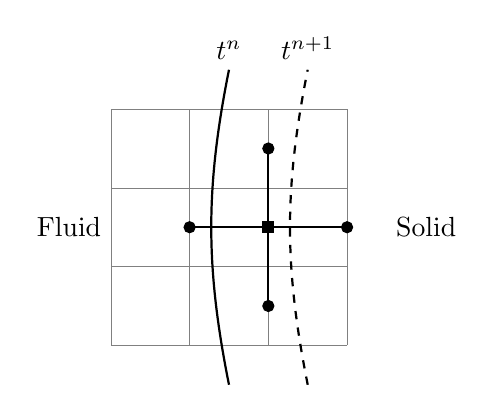
\begin{tikzpicture}

%grid
\draw[step=1cm,gray,very thin] (0,0) grid (3,3);

 %body 
\draw[black, thick] (1.5,-0.5) .. controls (1.2,1) and (1.2,2) .. (1.5,3.5) node[anchor=south] {$t^{n}$};
\draw[black, thick, dashed] (2.5,-0.5) .. controls (2.2,1) and (2.2,2) .. (2.5,3.5) node[anchor=south] {$t^{n+1}$};

%stencil
\filldraw ([xshift=-2pt,yshift=-2pt]2,1.5) rectangle ++(4pt,4pt);       %ghost node
\filldraw [black] (1,1.5) circle (2pt);
\filldraw [black] (3,1.5) circle (2pt);
\filldraw [black] (2,2.5) circle (2pt);
\filldraw [black] (2,0.5) circle (2pt);
\draw[black,thick] (1,1.5) -- (3,1.5);
\draw[black,thick] (2,0.5) -- (2,2.5);

%words
\node[anchor=east] at (0,1.5) {Fluid};
\node[anchor=west] at (3.5,1.5) {Solid};

\end{tikzpicture}


\end{document}
